
% Default to the notebook output style

    


% Inherit from the specified cell style.




    
\documentclass[11pt]{article}

    
    
    \usepackage[T1]{fontenc}
    % Nicer default font (+ math font) than Computer Modern for most use cases
    \usepackage{mathpazo}

    % Basic figure setup, for now with no caption control since it's done
    % automatically by Pandoc (which extracts ![](path) syntax from Markdown).
    \usepackage{graphicx}
    % We will generate all images so they have a width \maxwidth. This means
    % that they will get their normal width if they fit onto the page, but
    % are scaled down if they would overflow the margins.
    \makeatletter
    \def\maxwidth{\ifdim\Gin@nat@width>\linewidth\linewidth
    \else\Gin@nat@width\fi}
    \makeatother
    \let\Oldincludegraphics\includegraphics
    % Set max figure width to be 80% of text width, for now hardcoded.
    \renewcommand{\includegraphics}[1]{\Oldincludegraphics[width=.8\maxwidth]{#1}}
    % Ensure that by default, figures have no caption (until we provide a
    % proper Figure object with a Caption API and a way to capture that
    % in the conversion process - todo).
    \usepackage{caption}
    \DeclareCaptionLabelFormat{nolabel}{}
    \captionsetup{labelformat=nolabel}

    \usepackage{adjustbox} % Used to constrain images to a maximum size 
    \usepackage{xcolor} % Allow colors to be defined
    \usepackage{enumerate} % Needed for markdown enumerations to work
    \usepackage{geometry} % Used to adjust the document margins
    \usepackage{amsmath} % Equations
    \usepackage{amssymb} % Equations
    \usepackage{textcomp} % defines textquotesingle
    % Hack from http://tex.stackexchange.com/a/47451/13684:
    \AtBeginDocument{%
        \def\PYZsq{\textquotesingle}% Upright quotes in Pygmentized code
    }
    \usepackage{upquote} % Upright quotes for verbatim code
    \usepackage{eurosym} % defines \euro
    \usepackage[mathletters]{ucs} % Extended unicode (utf-8) support
    \usepackage[utf8x]{inputenc} % Allow utf-8 characters in the tex document
    \usepackage{fancyvrb} % verbatim replacement that allows latex
    \usepackage{grffile} % extends the file name processing of package graphics 
                         % to support a larger range 
    % The hyperref package gives us a pdf with properly built
    % internal navigation ('pdf bookmarks' for the table of contents,
    % internal cross-reference links, web links for URLs, etc.)
    \usepackage{hyperref}
    \usepackage{longtable} % longtable support required by pandoc >1.10
    \usepackage{booktabs}  % table support for pandoc > 1.12.2
    \usepackage[inline]{enumitem} % IRkernel/repr support (it uses the enumerate* environment)
    \usepackage[normalem]{ulem} % ulem is needed to support strikethroughs (\sout)
                                % normalem makes italics be italics, not underlines
    

    
    
    % Colors for the hyperref package
    \definecolor{urlcolor}{rgb}{0,.145,.698}
    \definecolor{linkcolor}{rgb}{.71,0.21,0.01}
    \definecolor{citecolor}{rgb}{.12,.54,.11}

    % ANSI colors
    \definecolor{ansi-black}{HTML}{3E424D}
    \definecolor{ansi-black-intense}{HTML}{282C36}
    \definecolor{ansi-red}{HTML}{E75C58}
    \definecolor{ansi-red-intense}{HTML}{B22B31}
    \definecolor{ansi-green}{HTML}{00A250}
    \definecolor{ansi-green-intense}{HTML}{007427}
    \definecolor{ansi-yellow}{HTML}{DDB62B}
    \definecolor{ansi-yellow-intense}{HTML}{B27D12}
    \definecolor{ansi-blue}{HTML}{208FFB}
    \definecolor{ansi-blue-intense}{HTML}{0065CA}
    \definecolor{ansi-magenta}{HTML}{D160C4}
    \definecolor{ansi-magenta-intense}{HTML}{A03196}
    \definecolor{ansi-cyan}{HTML}{60C6C8}
    \definecolor{ansi-cyan-intense}{HTML}{258F8F}
    \definecolor{ansi-white}{HTML}{C5C1B4}
    \definecolor{ansi-white-intense}{HTML}{A1A6B2}

    % commands and environments needed by pandoc snippets
    % extracted from the output of `pandoc -s`
    \providecommand{\tightlist}{%
      \setlength{\itemsep}{0pt}\setlength{\parskip}{0pt}}
    \DefineVerbatimEnvironment{Highlighting}{Verbatim}{commandchars=\\\{\}}
    % Add ',fontsize=\small' for more characters per line
    \newenvironment{Shaded}{}{}
    \newcommand{\KeywordTok}[1]{\textcolor[rgb]{0.00,0.44,0.13}{\textbf{{#1}}}}
    \newcommand{\DataTypeTok}[1]{\textcolor[rgb]{0.56,0.13,0.00}{{#1}}}
    \newcommand{\DecValTok}[1]{\textcolor[rgb]{0.25,0.63,0.44}{{#1}}}
    \newcommand{\BaseNTok}[1]{\textcolor[rgb]{0.25,0.63,0.44}{{#1}}}
    \newcommand{\FloatTok}[1]{\textcolor[rgb]{0.25,0.63,0.44}{{#1}}}
    \newcommand{\CharTok}[1]{\textcolor[rgb]{0.25,0.44,0.63}{{#1}}}
    \newcommand{\StringTok}[1]{\textcolor[rgb]{0.25,0.44,0.63}{{#1}}}
    \newcommand{\CommentTok}[1]{\textcolor[rgb]{0.38,0.63,0.69}{\textit{{#1}}}}
    \newcommand{\OtherTok}[1]{\textcolor[rgb]{0.00,0.44,0.13}{{#1}}}
    \newcommand{\AlertTok}[1]{\textcolor[rgb]{1.00,0.00,0.00}{\textbf{{#1}}}}
    \newcommand{\FunctionTok}[1]{\textcolor[rgb]{0.02,0.16,0.49}{{#1}}}
    \newcommand{\RegionMarkerTok}[1]{{#1}}
    \newcommand{\ErrorTok}[1]{\textcolor[rgb]{1.00,0.00,0.00}{\textbf{{#1}}}}
    \newcommand{\NormalTok}[1]{{#1}}
    
    % Additional commands for more recent versions of Pandoc
    \newcommand{\ConstantTok}[1]{\textcolor[rgb]{0.53,0.00,0.00}{{#1}}}
    \newcommand{\SpecialCharTok}[1]{\textcolor[rgb]{0.25,0.44,0.63}{{#1}}}
    \newcommand{\VerbatimStringTok}[1]{\textcolor[rgb]{0.25,0.44,0.63}{{#1}}}
    \newcommand{\SpecialStringTok}[1]{\textcolor[rgb]{0.73,0.40,0.53}{{#1}}}
    \newcommand{\ImportTok}[1]{{#1}}
    \newcommand{\DocumentationTok}[1]{\textcolor[rgb]{0.73,0.13,0.13}{\textit{{#1}}}}
    \newcommand{\AnnotationTok}[1]{\textcolor[rgb]{0.38,0.63,0.69}{\textbf{\textit{{#1}}}}}
    \newcommand{\CommentVarTok}[1]{\textcolor[rgb]{0.38,0.63,0.69}{\textbf{\textit{{#1}}}}}
    \newcommand{\VariableTok}[1]{\textcolor[rgb]{0.10,0.09,0.49}{{#1}}}
    \newcommand{\ControlFlowTok}[1]{\textcolor[rgb]{0.00,0.44,0.13}{\textbf{{#1}}}}
    \newcommand{\OperatorTok}[1]{\textcolor[rgb]{0.40,0.40,0.40}{{#1}}}
    \newcommand{\BuiltInTok}[1]{{#1}}
    \newcommand{\ExtensionTok}[1]{{#1}}
    \newcommand{\PreprocessorTok}[1]{\textcolor[rgb]{0.74,0.48,0.00}{{#1}}}
    \newcommand{\AttributeTok}[1]{\textcolor[rgb]{0.49,0.56,0.16}{{#1}}}
    \newcommand{\InformationTok}[1]{\textcolor[rgb]{0.38,0.63,0.69}{\textbf{\textit{{#1}}}}}
    \newcommand{\WarningTok}[1]{\textcolor[rgb]{0.38,0.63,0.69}{\textbf{\textit{{#1}}}}}
    
    
    % Define a nice break command that doesn't care if a line doesn't already
    % exist.
    \def\br{\hspace*{\fill} \\* }
    % Math Jax compatability definitions
    \def\gt{>}
    \def\lt{<}
    % Document parameters
    \title{hw3}
    
    
    

    % Pygments definitions
    
\makeatletter
\def\PY@reset{\let\PY@it=\relax \let\PY@bf=\relax%
    \let\PY@ul=\relax \let\PY@tc=\relax%
    \let\PY@bc=\relax \let\PY@ff=\relax}
\def\PY@tok#1{\csname PY@tok@#1\endcsname}
\def\PY@toks#1+{\ifx\relax#1\empty\else%
    \PY@tok{#1}\expandafter\PY@toks\fi}
\def\PY@do#1{\PY@bc{\PY@tc{\PY@ul{%
    \PY@it{\PY@bf{\PY@ff{#1}}}}}}}
\def\PY#1#2{\PY@reset\PY@toks#1+\relax+\PY@do{#2}}

\expandafter\def\csname PY@tok@w\endcsname{\def\PY@tc##1{\textcolor[rgb]{0.73,0.73,0.73}{##1}}}
\expandafter\def\csname PY@tok@c\endcsname{\let\PY@it=\textit\def\PY@tc##1{\textcolor[rgb]{0.25,0.50,0.50}{##1}}}
\expandafter\def\csname PY@tok@cp\endcsname{\def\PY@tc##1{\textcolor[rgb]{0.74,0.48,0.00}{##1}}}
\expandafter\def\csname PY@tok@k\endcsname{\let\PY@bf=\textbf\def\PY@tc##1{\textcolor[rgb]{0.00,0.50,0.00}{##1}}}
\expandafter\def\csname PY@tok@kp\endcsname{\def\PY@tc##1{\textcolor[rgb]{0.00,0.50,0.00}{##1}}}
\expandafter\def\csname PY@tok@kt\endcsname{\def\PY@tc##1{\textcolor[rgb]{0.69,0.00,0.25}{##1}}}
\expandafter\def\csname PY@tok@o\endcsname{\def\PY@tc##1{\textcolor[rgb]{0.40,0.40,0.40}{##1}}}
\expandafter\def\csname PY@tok@ow\endcsname{\let\PY@bf=\textbf\def\PY@tc##1{\textcolor[rgb]{0.67,0.13,1.00}{##1}}}
\expandafter\def\csname PY@tok@nb\endcsname{\def\PY@tc##1{\textcolor[rgb]{0.00,0.50,0.00}{##1}}}
\expandafter\def\csname PY@tok@nf\endcsname{\def\PY@tc##1{\textcolor[rgb]{0.00,0.00,1.00}{##1}}}
\expandafter\def\csname PY@tok@nc\endcsname{\let\PY@bf=\textbf\def\PY@tc##1{\textcolor[rgb]{0.00,0.00,1.00}{##1}}}
\expandafter\def\csname PY@tok@nn\endcsname{\let\PY@bf=\textbf\def\PY@tc##1{\textcolor[rgb]{0.00,0.00,1.00}{##1}}}
\expandafter\def\csname PY@tok@ne\endcsname{\let\PY@bf=\textbf\def\PY@tc##1{\textcolor[rgb]{0.82,0.25,0.23}{##1}}}
\expandafter\def\csname PY@tok@nv\endcsname{\def\PY@tc##1{\textcolor[rgb]{0.10,0.09,0.49}{##1}}}
\expandafter\def\csname PY@tok@no\endcsname{\def\PY@tc##1{\textcolor[rgb]{0.53,0.00,0.00}{##1}}}
\expandafter\def\csname PY@tok@nl\endcsname{\def\PY@tc##1{\textcolor[rgb]{0.63,0.63,0.00}{##1}}}
\expandafter\def\csname PY@tok@ni\endcsname{\let\PY@bf=\textbf\def\PY@tc##1{\textcolor[rgb]{0.60,0.60,0.60}{##1}}}
\expandafter\def\csname PY@tok@na\endcsname{\def\PY@tc##1{\textcolor[rgb]{0.49,0.56,0.16}{##1}}}
\expandafter\def\csname PY@tok@nt\endcsname{\let\PY@bf=\textbf\def\PY@tc##1{\textcolor[rgb]{0.00,0.50,0.00}{##1}}}
\expandafter\def\csname PY@tok@nd\endcsname{\def\PY@tc##1{\textcolor[rgb]{0.67,0.13,1.00}{##1}}}
\expandafter\def\csname PY@tok@s\endcsname{\def\PY@tc##1{\textcolor[rgb]{0.73,0.13,0.13}{##1}}}
\expandafter\def\csname PY@tok@sd\endcsname{\let\PY@it=\textit\def\PY@tc##1{\textcolor[rgb]{0.73,0.13,0.13}{##1}}}
\expandafter\def\csname PY@tok@si\endcsname{\let\PY@bf=\textbf\def\PY@tc##1{\textcolor[rgb]{0.73,0.40,0.53}{##1}}}
\expandafter\def\csname PY@tok@se\endcsname{\let\PY@bf=\textbf\def\PY@tc##1{\textcolor[rgb]{0.73,0.40,0.13}{##1}}}
\expandafter\def\csname PY@tok@sr\endcsname{\def\PY@tc##1{\textcolor[rgb]{0.73,0.40,0.53}{##1}}}
\expandafter\def\csname PY@tok@ss\endcsname{\def\PY@tc##1{\textcolor[rgb]{0.10,0.09,0.49}{##1}}}
\expandafter\def\csname PY@tok@sx\endcsname{\def\PY@tc##1{\textcolor[rgb]{0.00,0.50,0.00}{##1}}}
\expandafter\def\csname PY@tok@m\endcsname{\def\PY@tc##1{\textcolor[rgb]{0.40,0.40,0.40}{##1}}}
\expandafter\def\csname PY@tok@gh\endcsname{\let\PY@bf=\textbf\def\PY@tc##1{\textcolor[rgb]{0.00,0.00,0.50}{##1}}}
\expandafter\def\csname PY@tok@gu\endcsname{\let\PY@bf=\textbf\def\PY@tc##1{\textcolor[rgb]{0.50,0.00,0.50}{##1}}}
\expandafter\def\csname PY@tok@gd\endcsname{\def\PY@tc##1{\textcolor[rgb]{0.63,0.00,0.00}{##1}}}
\expandafter\def\csname PY@tok@gi\endcsname{\def\PY@tc##1{\textcolor[rgb]{0.00,0.63,0.00}{##1}}}
\expandafter\def\csname PY@tok@gr\endcsname{\def\PY@tc##1{\textcolor[rgb]{1.00,0.00,0.00}{##1}}}
\expandafter\def\csname PY@tok@ge\endcsname{\let\PY@it=\textit}
\expandafter\def\csname PY@tok@gs\endcsname{\let\PY@bf=\textbf}
\expandafter\def\csname PY@tok@gp\endcsname{\let\PY@bf=\textbf\def\PY@tc##1{\textcolor[rgb]{0.00,0.00,0.50}{##1}}}
\expandafter\def\csname PY@tok@go\endcsname{\def\PY@tc##1{\textcolor[rgb]{0.53,0.53,0.53}{##1}}}
\expandafter\def\csname PY@tok@gt\endcsname{\def\PY@tc##1{\textcolor[rgb]{0.00,0.27,0.87}{##1}}}
\expandafter\def\csname PY@tok@err\endcsname{\def\PY@bc##1{\setlength{\fboxsep}{0pt}\fcolorbox[rgb]{1.00,0.00,0.00}{1,1,1}{\strut ##1}}}
\expandafter\def\csname PY@tok@kc\endcsname{\let\PY@bf=\textbf\def\PY@tc##1{\textcolor[rgb]{0.00,0.50,0.00}{##1}}}
\expandafter\def\csname PY@tok@kd\endcsname{\let\PY@bf=\textbf\def\PY@tc##1{\textcolor[rgb]{0.00,0.50,0.00}{##1}}}
\expandafter\def\csname PY@tok@kn\endcsname{\let\PY@bf=\textbf\def\PY@tc##1{\textcolor[rgb]{0.00,0.50,0.00}{##1}}}
\expandafter\def\csname PY@tok@kr\endcsname{\let\PY@bf=\textbf\def\PY@tc##1{\textcolor[rgb]{0.00,0.50,0.00}{##1}}}
\expandafter\def\csname PY@tok@bp\endcsname{\def\PY@tc##1{\textcolor[rgb]{0.00,0.50,0.00}{##1}}}
\expandafter\def\csname PY@tok@fm\endcsname{\def\PY@tc##1{\textcolor[rgb]{0.00,0.00,1.00}{##1}}}
\expandafter\def\csname PY@tok@vc\endcsname{\def\PY@tc##1{\textcolor[rgb]{0.10,0.09,0.49}{##1}}}
\expandafter\def\csname PY@tok@vg\endcsname{\def\PY@tc##1{\textcolor[rgb]{0.10,0.09,0.49}{##1}}}
\expandafter\def\csname PY@tok@vi\endcsname{\def\PY@tc##1{\textcolor[rgb]{0.10,0.09,0.49}{##1}}}
\expandafter\def\csname PY@tok@vm\endcsname{\def\PY@tc##1{\textcolor[rgb]{0.10,0.09,0.49}{##1}}}
\expandafter\def\csname PY@tok@sa\endcsname{\def\PY@tc##1{\textcolor[rgb]{0.73,0.13,0.13}{##1}}}
\expandafter\def\csname PY@tok@sb\endcsname{\def\PY@tc##1{\textcolor[rgb]{0.73,0.13,0.13}{##1}}}
\expandafter\def\csname PY@tok@sc\endcsname{\def\PY@tc##1{\textcolor[rgb]{0.73,0.13,0.13}{##1}}}
\expandafter\def\csname PY@tok@dl\endcsname{\def\PY@tc##1{\textcolor[rgb]{0.73,0.13,0.13}{##1}}}
\expandafter\def\csname PY@tok@s2\endcsname{\def\PY@tc##1{\textcolor[rgb]{0.73,0.13,0.13}{##1}}}
\expandafter\def\csname PY@tok@sh\endcsname{\def\PY@tc##1{\textcolor[rgb]{0.73,0.13,0.13}{##1}}}
\expandafter\def\csname PY@tok@s1\endcsname{\def\PY@tc##1{\textcolor[rgb]{0.73,0.13,0.13}{##1}}}
\expandafter\def\csname PY@tok@mb\endcsname{\def\PY@tc##1{\textcolor[rgb]{0.40,0.40,0.40}{##1}}}
\expandafter\def\csname PY@tok@mf\endcsname{\def\PY@tc##1{\textcolor[rgb]{0.40,0.40,0.40}{##1}}}
\expandafter\def\csname PY@tok@mh\endcsname{\def\PY@tc##1{\textcolor[rgb]{0.40,0.40,0.40}{##1}}}
\expandafter\def\csname PY@tok@mi\endcsname{\def\PY@tc##1{\textcolor[rgb]{0.40,0.40,0.40}{##1}}}
\expandafter\def\csname PY@tok@il\endcsname{\def\PY@tc##1{\textcolor[rgb]{0.40,0.40,0.40}{##1}}}
\expandafter\def\csname PY@tok@mo\endcsname{\def\PY@tc##1{\textcolor[rgb]{0.40,0.40,0.40}{##1}}}
\expandafter\def\csname PY@tok@ch\endcsname{\let\PY@it=\textit\def\PY@tc##1{\textcolor[rgb]{0.25,0.50,0.50}{##1}}}
\expandafter\def\csname PY@tok@cm\endcsname{\let\PY@it=\textit\def\PY@tc##1{\textcolor[rgb]{0.25,0.50,0.50}{##1}}}
\expandafter\def\csname PY@tok@cpf\endcsname{\let\PY@it=\textit\def\PY@tc##1{\textcolor[rgb]{0.25,0.50,0.50}{##1}}}
\expandafter\def\csname PY@tok@c1\endcsname{\let\PY@it=\textit\def\PY@tc##1{\textcolor[rgb]{0.25,0.50,0.50}{##1}}}
\expandafter\def\csname PY@tok@cs\endcsname{\let\PY@it=\textit\def\PY@tc##1{\textcolor[rgb]{0.25,0.50,0.50}{##1}}}

\def\PYZbs{\char`\\}
\def\PYZus{\char`\_}
\def\PYZob{\char`\{}
\def\PYZcb{\char`\}}
\def\PYZca{\char`\^}
\def\PYZam{\char`\&}
\def\PYZlt{\char`\<}
\def\PYZgt{\char`\>}
\def\PYZsh{\char`\#}
\def\PYZpc{\char`\%}
\def\PYZdl{\char`\$}
\def\PYZhy{\char`\-}
\def\PYZsq{\char`\'}
\def\PYZdq{\char`\"}
\def\PYZti{\char`\~}
% for compatibility with earlier versions
\def\PYZat{@}
\def\PYZlb{[}
\def\PYZrb{]}
\makeatother


    % Exact colors from NB
    \definecolor{incolor}{rgb}{0.0, 0.0, 0.5}
    \definecolor{outcolor}{rgb}{0.545, 0.0, 0.0}



    
    % Prevent overflowing lines due to hard-to-break entities
    \sloppy 
    % Setup hyperref package
    \hypersetup{
      breaklinks=true,  % so long urls are correctly broken across lines
      colorlinks=true,
      urlcolor=urlcolor,
      linkcolor=linkcolor,
      citecolor=citecolor,
      }
    % Slightly bigger margins than the latex defaults
    
    \geometry{verbose,tmargin=1in,bmargin=1in,lmargin=1in,rmargin=1in}
    
    

    \begin{document}
    
    
    \maketitle
    
    

    
    \hypertarget{section}{%
\subsection{2.49}\label{section}}

\hypertarget{a}{%
\subsubsection{a)}\label{a}}

Yes. Consider the following setting:

Denote \(A= \begin{bmatrix}1 & -1 \\ 1 & -1\end{bmatrix}\) and
\(b=(1,-1)^T\). Then the set \(\{x|Ax \leq b; x\geq 0\}\) is empty while
the set \(\{d|Ad\leq 0; d\geq 0, 1^Td=0\}\) has a element of
\((0.5, 0.5)^T\).

\hypertarget{b}{%
\subsubsection{b)}\label{b}}

There's no relationship between these two. The left figure has a
redundant defining plane (1), but has no degeneracy. While the second
figure has 1 degree of degeneracy, but has no redundancy.

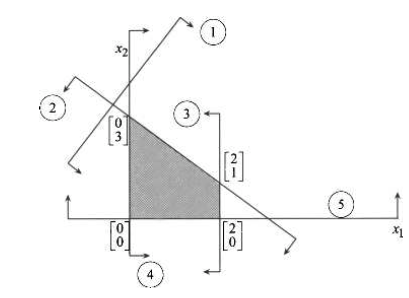
\includegraphics{./figs/redundancy.png}
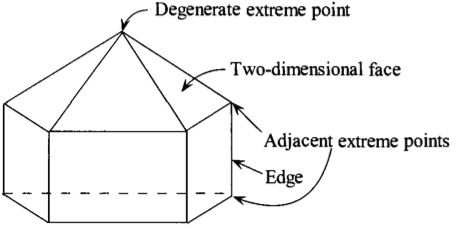
\includegraphics{./figs/degenercy.png}

\hypertarget{c}{%
\subsubsection{c)}\label{c}}

Yes. Because in three dimensions or higher, a degenerated extreme point
can lie on more than 2 defining planes and remove any of it will change
the polyhedron set while it is not true for 2-d space.

\hypertarget{d}{%
\subsubsection{d)}\label{d}}

No.~Consider \(A= \begin{bmatrix}1 & 0 \\ 1 & 0\end{bmatrix}\) and
\(b=(2, 1)^T\) and the polyhedron set defined by \(A\) and \(b\), that
is \(\{x|Ax \leq b\}\). The intersection of two half spaces is
\(\{(x,y); x\leq 1, y\in R\}\), but there is no extreme point.

\hypertarget{e}{%
\subsubsection{e)}\label{e}}

False. Consider a convex cone defined by \(n+1\) hyper-planes, then it
can have \(n+1\) extreme directions. For example, the figure below has
more than 3 extreme directions. (Source:Google Image.)

\begin{figure}
\centering
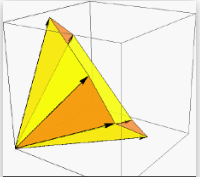
\includegraphics{./figs/cone.png}
\caption{(a)}
\end{figure}

\hypertarget{f}{%
\subsubsection{f)}\label{f}}

dim(X) = n - r.

    \hypertarget{section}{%
\subsection{2.50}\label{section}}

We can have at most \(C_6^4=15\) basic solutions. By the code following,
we see there are only 13 basic solutions. Out of 13 basic solutions,
there are only 4 basic feasible solutions, which implies we have 4
extreme points.

Extreme points are:

\begin{verbatim}
(0,1,0,1), (0,1,0,0), (0,0,0,1), (0,0,0,0)
\end{verbatim}

    \begin{Verbatim}[commandchars=\\\{\}]
{\color{incolor}In [{\color{incolor}19}]:} \PY{k+kn}{import} \PY{n+nn}{numpy} \PY{k}{as} \PY{n+nn}{np}
         \PY{n}{A} \PY{o}{=} \PY{n}{np}\PY{o}{.}\PY{n}{array}\PY{p}{(}\PY{p}{[}\PY{p}{[}\PY{o}{\PYZhy{}}\PY{l+m+mi}{1}\PY{p}{,}\PY{l+m+mi}{1}\PY{p}{,}\PY{o}{\PYZhy{}}\PY{l+m+mi}{2}\PY{p}{,}\PY{l+m+mi}{0}\PY{p}{]}\PY{p}{,} \PY{p}{[}\PY{o}{\PYZhy{}}\PY{l+m+mi}{2}\PY{p}{,}\PY{l+m+mi}{0}\PY{p}{,}\PY{o}{\PYZhy{}}\PY{l+m+mi}{1}\PY{p}{,}\PY{l+m+mi}{2}\PY{p}{]}\PY{p}{,} \PY{p}{[}\PY{l+m+mi}{1}\PY{p}{,}\PY{l+m+mi}{0}\PY{p}{,}\PY{l+m+mi}{0}\PY{p}{,}\PY{l+m+mi}{0}\PY{p}{]}\PY{p}{,} \PY{p}{[}\PY{l+m+mi}{0}\PY{p}{,}\PY{l+m+mi}{1}\PY{p}{,}\PY{l+m+mi}{0}\PY{p}{,}\PY{l+m+mi}{0}\PY{p}{]}\PY{p}{,} \PY{p}{[}\PY{l+m+mi}{0}\PY{p}{,}\PY{l+m+mi}{0}\PY{p}{,}\PY{l+m+mi}{1}\PY{p}{,}\PY{l+m+mi}{0}\PY{p}{]}\PY{p}{,} \PY{p}{[}\PY{l+m+mi}{0}\PY{p}{,}\PY{l+m+mi}{0}\PY{p}{,}\PY{l+m+mi}{0}\PY{p}{,}\PY{l+m+mi}{1}\PY{p}{]}\PY{p}{]}\PY{p}{)}
         \PY{n}{b} \PY{o}{=} \PY{n}{np}\PY{o}{.}\PY{n}{array}\PY{p}{(}\PY{p}{[}\PY{p}{[}\PY{l+m+mi}{1}\PY{p}{]}\PY{p}{,}\PY{p}{[}\PY{l+m+mi}{2}\PY{p}{]}\PY{p}{,}\PY{p}{[}\PY{l+m+mi}{0}\PY{p}{]}\PY{p}{,}\PY{p}{[}\PY{l+m+mi}{0}\PY{p}{]}\PY{p}{,}\PY{p}{[}\PY{l+m+mi}{0}\PY{p}{]}\PY{p}{,}\PY{p}{[}\PY{l+m+mi}{0}\PY{p}{]}\PY{p}{]}\PY{p}{)}
         \PY{n}{root} \PY{o}{=} \PY{p}{\PYZob{}}\PY{p}{\PYZcb{}}
         \PY{k}{for} \PY{n}{i} \PY{o+ow}{in} \PY{n+nb}{range}\PY{p}{(}\PY{l+m+mi}{0}\PY{p}{,} \PY{n}{A}\PY{o}{.}\PY{n}{shape}\PY{p}{[}\PY{l+m+mi}{0}\PY{p}{]}\PY{o}{\PYZhy{}}\PY{l+m+mi}{3}\PY{p}{)}\PY{p}{:}
             \PY{k}{for} \PY{n}{j} \PY{o+ow}{in} \PY{n+nb}{range}\PY{p}{(}\PY{n}{i}\PY{o}{+}\PY{l+m+mi}{1}\PY{p}{,} \PY{n}{A}\PY{o}{.}\PY{n}{shape}\PY{p}{[}\PY{l+m+mi}{0}\PY{p}{]}\PY{o}{\PYZhy{}}\PY{l+m+mi}{2}\PY{p}{)}\PY{p}{:}
                 \PY{k}{for} \PY{n}{k} \PY{o+ow}{in} \PY{n+nb}{range}\PY{p}{(}\PY{n}{j}\PY{o}{+}\PY{l+m+mi}{1}\PY{p}{,} \PY{n}{A}\PY{o}{.}\PY{n}{shape}\PY{p}{[}\PY{l+m+mi}{0}\PY{p}{]}\PY{o}{\PYZhy{}}\PY{l+m+mi}{1}\PY{p}{)}\PY{p}{:}
                     \PY{k}{for} \PY{n}{l} \PY{o+ow}{in} \PY{n+nb}{range}\PY{p}{(}\PY{n}{k}\PY{o}{+}\PY{l+m+mi}{1}\PY{p}{,} \PY{n}{A}\PY{o}{.}\PY{n}{shape}\PY{p}{[}\PY{l+m+mi}{0}\PY{p}{]}\PY{p}{)}\PY{p}{:}
                         \PY{k}{try}\PY{p}{:} 
                             \PY{n}{temp} \PY{o}{=} \PY{n}{np}\PY{o}{.}\PY{n}{linalg}\PY{o}{.}\PY{n}{solve}\PY{p}{(}\PY{n}{A}\PY{p}{[}\PY{p}{[}\PY{n}{i}\PY{p}{,}\PY{n}{j}\PY{p}{,}\PY{n}{k}\PY{p}{,}\PY{n}{l}\PY{p}{]}\PY{p}{,} \PY{p}{:}\PY{p}{]}\PY{p}{,} \PY{n}{b}\PY{p}{[}\PY{p}{[}\PY{n}{i}\PY{p}{,}\PY{n}{j}\PY{p}{,}\PY{n}{k}\PY{p}{,}\PY{n}{l}\PY{p}{]}\PY{p}{,}\PY{p}{:}\PY{p}{]}\PY{p}{)}
                             \PY{n}{root}\PY{p}{[}\PY{n+nb}{str}\PY{p}{(}\PY{n}{i}\PY{p}{)}\PY{o}{+}\PY{n+nb}{str}\PY{p}{(}\PY{n}{j}\PY{p}{)}\PY{o}{+}\PY{n+nb}{str}\PY{p}{(}\PY{n}{k}\PY{p}{)}\PY{o}{+}\PY{n+nb}{str}\PY{p}{(}\PY{n}{l}\PY{p}{)}\PY{p}{]} \PY{o}{=} \PY{n}{temp}
                         \PY{k}{except} \PY{n}{np}\PY{o}{.}\PY{n}{linalg}\PY{o}{.}\PY{n}{LinAlgError}\PY{p}{:}
                             \PY{k}{pass}
\end{Verbatim}


    To find the extreme directions, it's equivalent to find the basic
feasible solutions of the \(\{d | Ad\leq 0, d\geq 0\ 1^Td=0\}\).

Extreme directions are:

\begin{verbatim}
(0, 4/7, 2/7, 1/7)
(1/3, 1/3, 0, 1/3), (0, 0, 2/3, 1/3), (0, 2/3, 1/3, 0)
(0.5, 0, 0, 0.5), (0.5, 0.5, 0, 0)
(1,0,0,0), (0, 1, 0, 0), (0, 0, 1, 0), (0,0,0,1)
\end{verbatim}

    \begin{Verbatim}[commandchars=\\\{\}]
{\color{incolor}In [{\color{incolor}2}]:} \PY{n}{A} \PY{o}{=} \PY{n}{np}\PY{o}{.}\PY{n}{array}\PY{p}{(}\PY{p}{[}\PY{p}{[}\PY{o}{\PYZhy{}}\PY{l+m+mi}{1}\PY{p}{,}\PY{l+m+mi}{1}\PY{p}{,}\PY{o}{\PYZhy{}}\PY{l+m+mi}{2}\PY{p}{,}\PY{l+m+mi}{0}\PY{p}{]}\PY{p}{,} \PY{p}{[}\PY{o}{\PYZhy{}}\PY{l+m+mi}{2}\PY{p}{,}\PY{l+m+mi}{0}\PY{p}{,}\PY{o}{\PYZhy{}}\PY{l+m+mi}{1}\PY{p}{,}\PY{l+m+mi}{2}\PY{p}{]}\PY{p}{,} \PY{p}{[}\PY{l+m+mi}{1}\PY{p}{,}\PY{l+m+mi}{0}\PY{p}{,}\PY{l+m+mi}{0}\PY{p}{,}\PY{l+m+mi}{0}\PY{p}{]}\PY{p}{,} \PY{p}{[}\PY{l+m+mi}{0}\PY{p}{,}\PY{l+m+mi}{1}\PY{p}{,}\PY{l+m+mi}{0}\PY{p}{,}\PY{l+m+mi}{0}\PY{p}{]}\PY{p}{,} \PY{p}{[}\PY{l+m+mi}{0}\PY{p}{,}\PY{l+m+mi}{0}\PY{p}{,}\PY{l+m+mi}{1}\PY{p}{,}\PY{l+m+mi}{0}\PY{p}{]}\PY{p}{,} \PY{p}{[}\PY{l+m+mi}{0}\PY{p}{,}\PY{l+m+mi}{0}\PY{p}{,}\PY{l+m+mi}{0}\PY{p}{,}\PY{l+m+mi}{1}\PY{p}{]}\PY{p}{,} \PY{p}{[}\PY{l+m+mi}{1}\PY{p}{,}\PY{l+m+mi}{1}\PY{p}{,}\PY{l+m+mi}{1}\PY{p}{,}\PY{l+m+mi}{1}\PY{p}{]}\PY{p}{]}\PY{p}{)}
        \PY{n}{zero} \PY{o}{=} \PY{n}{np}\PY{o}{.}\PY{n}{array}\PY{p}{(}\PY{p}{[}\PY{p}{[}\PY{l+m+mi}{0}\PY{p}{]}\PY{p}{,}\PY{p}{[}\PY{l+m+mi}{0}\PY{p}{]}\PY{p}{,}\PY{p}{[}\PY{l+m+mi}{0}\PY{p}{]}\PY{p}{,}\PY{p}{[}\PY{l+m+mi}{0}\PY{p}{]}\PY{p}{,}\PY{p}{[}\PY{l+m+mi}{0}\PY{p}{]}\PY{p}{,}\PY{p}{[}\PY{l+m+mi}{0}\PY{p}{]}\PY{p}{,}\PY{p}{[}\PY{l+m+mi}{1}\PY{p}{]}\PY{p}{]}\PY{p}{)}
        \PY{n}{root} \PY{o}{=} \PY{p}{\PYZob{}}\PY{p}{\PYZcb{}}
        \PY{k}{for} \PY{n}{i} \PY{o+ow}{in} \PY{n+nb}{range}\PY{p}{(}\PY{l+m+mi}{0}\PY{p}{,} \PY{n}{A}\PY{o}{.}\PY{n}{shape}\PY{p}{[}\PY{l+m+mi}{0}\PY{p}{]}\PY{o}{\PYZhy{}}\PY{l+m+mi}{3}\PY{p}{)}\PY{p}{:}
            \PY{k}{for} \PY{n}{j} \PY{o+ow}{in} \PY{n+nb}{range}\PY{p}{(}\PY{n}{i}\PY{o}{+}\PY{l+m+mi}{1}\PY{p}{,} \PY{n}{A}\PY{o}{.}\PY{n}{shape}\PY{p}{[}\PY{l+m+mi}{0}\PY{p}{]}\PY{o}{\PYZhy{}}\PY{l+m+mi}{2}\PY{p}{)}\PY{p}{:}
                \PY{k}{for} \PY{n}{k} \PY{o+ow}{in} \PY{n+nb}{range}\PY{p}{(}\PY{n}{j}\PY{o}{+}\PY{l+m+mi}{1}\PY{p}{,} \PY{n}{A}\PY{o}{.}\PY{n}{shape}\PY{p}{[}\PY{l+m+mi}{0}\PY{p}{]}\PY{o}{\PYZhy{}}\PY{l+m+mi}{1}\PY{p}{)}\PY{p}{:}
                        \PY{k}{try}\PY{p}{:} 
                            \PY{n}{temp} \PY{o}{=} \PY{n}{np}\PY{o}{.}\PY{n}{linalg}\PY{o}{.}\PY{n}{solve}\PY{p}{(}\PY{n}{A}\PY{p}{[}\PY{p}{[}\PY{n}{i}\PY{p}{,}\PY{n}{j}\PY{p}{,}\PY{n}{k}\PY{p}{,}\PY{l+m+mi}{6}\PY{p}{]}\PY{p}{,} \PY{p}{:}\PY{p}{]}\PY{p}{,} \PY{n}{zero}\PY{p}{[}\PY{p}{[}\PY{n}{i}\PY{p}{,}\PY{n}{j}\PY{p}{,}\PY{n}{k}\PY{p}{,}\PY{l+m+mi}{6}\PY{p}{]}\PY{p}{,}\PY{p}{:}\PY{p}{]}\PY{p}{)}
                            \PY{n}{check} \PY{o}{=} \PY{k+kc}{True}
                            \PY{k}{if} \PY{n}{np}\PY{o}{.}\PY{n}{sum}\PY{p}{(}\PY{p}{[}\PY{n}{d}\PY{o}{\PYZlt{}}\PY{l+m+mi}{0} \PY{k}{for} \PY{n}{d} \PY{o+ow}{in} \PY{n}{temp}\PY{p}{]}\PY{p}{)} \PY{o}{\PYZgt{}} \PY{l+m+mi}{0}\PY{p}{:}
                                \PY{n}{check} \PY{o}{=} \PY{k+kc}{False}
                            \PY{k}{if} \PY{n}{check}\PY{p}{:}
                                \PY{n}{root}\PY{p}{[}\PY{n+nb}{str}\PY{p}{(}\PY{n}{i}\PY{p}{)}\PY{o}{+}\PY{n+nb}{str}\PY{p}{(}\PY{n}{j}\PY{p}{)}\PY{o}{+}\PY{n+nb}{str}\PY{p}{(}\PY{n}{k}\PY{p}{)}\PY{o}{+}\PY{n+nb}{str}\PY{p}{(}\PY{l+m+mi}{6}\PY{p}{)}\PY{p}{]} \PY{o}{=} \PY{p}{[}\PY{n+nb}{float}\PY{p}{(}\PY{n}{x}\PY{p}{)}\PY{o}{.}\PY{n}{as\PYZus{}integer\PYZus{}ratio}\PY{p}{(}\PY{p}{)} \PY{k}{for} \PY{n}{x} \PY{o+ow}{in} \PY{n}{temp}\PY{p}{]}
                        \PY{k}{except} \PY{n}{np}\PY{o}{.}\PY{n}{linalg}\PY{o}{.}\PY{n}{LinAlgError}\PY{p}{:}
                            \PY{k}{pass}
\end{Verbatim}


    \hypertarget{exercise-2.6}{%
\subsection{Exercise 2.6}\label{exercise-2.6}}

\begin{enumerate}
\def\labelenumi{\alph{enumi})}
\tightlist
\item
  If \(n\leq m\), then the argument is trivial. Now suppose that
  \(n>m+1\). Pick an arbitrary \(y\in C\) and consider the polyhedral
  set
\end{enumerate}

\[
P = \{\lambda=(\lambda_1,...\lambda_n)| \sum_{i=1}^m \lambda_i A_i=y\}.
\]

By the choice of \(y\), we know that there exist an extreme point in
P,say \(x_0\) (corollary 2.2). So there are at least \(n-m\) zero
components in \(\lambda\), which implies that there are at most \(m\)
nonzero components in \(\lambda\). This concludes the proof.

\begin{enumerate}
\def\labelenumi{\alph{enumi})}
\setcounter{enumi}{1}
\item
\end{enumerate}

If \(n\leq m\), then the argument is trivial.Now suppose that \(n>m+1\).
Pick an arbitrary \(y\in C\) and consider the polyhedral set

\[
P = \{\lambda=(\lambda_1,...\lambda_n)| \sum_{i=1}^m \lambda_i A_i=y, \sum_{i=1}^n \lambda_i = 1\}.
\]

By the choice of \(y\), we know that there exist an extreme point in
P,say \(x_0\) (corollary 2.2). So there are at least \(n-m-1\) zero
components in \(\lambda\), which implies that there are at most \(m+1\)
nonzero components in \(\lambda\). This concludes the proof.

    \hypertarget{exercise-2.10}{%
\subsection{Exercise 2.10}\label{exercise-2.10}}

\begin{enumerate}
\def\labelenumi{\alph{enumi})}
\tightlist
\item
  \textbf{TRUE}
\end{enumerate}

proof: WLOG, we assume \(A=[A_1, A_2], x=(x_1,x_2)^T\), where
\(A_1, A_2, x_1, x_2\) are of dimension
\(m\times m, m\times 1, m\times 1, 1\times 1\) and \(A_1\) are of rank
\(m\). Then we can rewrite \(Ax=b\) as \(A_1x_1 + A_2x_2=b\). As \(A_1\)
is invertible, \(x_1=A_1^{-1}(b-A_2x_2)\), which implies the dimension
of \(X\) is actually 1. That is to say, the solutions are always of the
form \[
x= \begin{bmatrix}A_1^{-1}(b-A_2x_2) \\ x_2\end{bmatrix} \overset{\Delta}{=} \begin{bmatrix}a-cx_2 \\ x_2\end{bmatrix} 
\] Note that if we have more than two basic feasible solution, say
three, then they must lie on a line segment, which is contained with the
\(X\). Then the ``middle'' one can be represent as a strict convex
combination of the remaining two, which leads to the contradiction of
the definition of the extreme point.

\begin{enumerate}
\def\labelenumi{\alph{enumi})}
\setcounter{enumi}{1}
\tightlist
\item
  \textbf{False}
\end{enumerate}

Consider minimizing \(0\), subject to \(x\geq 0\). The optimal solution
set \([0, \infty)\) is unbounded.

\begin{enumerate}
\def\labelenumi{\alph{enumi})}
\setcounter{enumi}{2}
\tightlist
\item
  \textbf{False}
\end{enumerate}

Consider the problem \[
\min_{x\in X} 0, 
\]

then all \(x\in X\) are optimal, but they are not necessarily to be a
basic feasible solution.

\begin{enumerate}
\def\labelenumi{\alph{enumi})}
\setcounter{enumi}{3}
\tightlist
\item
  \textbf{True}
\end{enumerate}

The convex combination of any two optimal is another optimal solution.

\begin{enumerate}
\def\labelenumi{\alph{enumi})}
\setcounter{enumi}{4}
\tightlist
\item
  \textbf{False}
\end{enumerate}

\[
\begin{align*}
& \min_{x_2} x_2 \\
& s.t. \\
& x_3 = 1 \\
& x_1, x_2, x_3 \geq 0
\end{align*}
\]

Then the optimal solution set is \(\{(x_1,0,0)|x_1 \geq 0\}\). But we
only have one basic feasible solution set.

\begin{enumerate}
\def\labelenumi{\alph{enumi})}
\setcounter{enumi}{5}
\tightlist
\item
  \textbf{False}
\end{enumerate}

Consider the following problem:

\[
\begin{align*}
& \min_{x_1,x_2} \max\{x_1-x_2, x_2-x_1\} \\
& s.t. \\
& x_2 = 1 \\
& x_1 + x_3 = 2\\
& x_1, x_2, x_3 \geq 0
\end{align*}
\] \((1, 1, 1)\) is the unique optimal solution, but there are only two
constraints that are active at \((1, 1, 1)\).

    \hypertarget{exercise-2.12}{%
\subsection{Exercise 2.12}\label{exercise-2.12}}

True. The point \(x_0=(0,0,...,0)^T\) is a basic feasible solution.

    \hypertarget{exercise-2.13}{%
\subsection{Exercise 2.13}\label{exercise-2.13}}

\hypertarget{a}{%
\subsubsection{(a)}\label{a}}

We proof this by using contradiction. WLOG, we assume
\(x=(x_1,...,x_m,0,...,0)^T\), where \(x_1,...,x_m >0\), and partition
\(A\) according to \(x\) as \(A=[A_M,A_Z]\), where \(A_M\) is a \(m*m\)
matrix.

Suppose \(x\) is not a basic feasible solution, then we know that the
following \(n*n\) matrix's rank is less than n. \[
B=
\begin{bmatrix}
A_M & A_Z\\
0 & I_{(n-m)\times (n-m)}
\end{bmatrix}
\] To simplify the analysis, let's assume that \(r(B)=n-1\) and the
\(m\)-th row of \(B\) can be write as a non-trivial linear combination
of the rest of n-1 rows. Denote \(A_{M-1}\) and \(A_{Z-1}\) as the
\(A_M\) and \(A_Z\) without the \(m\)-th row.

Consider the equation \[
\begin{bmatrix}
A_{M-1} & A_{Z-1}\\
0 & I_{(n-m+1)\times (n-m+1)}
\end{bmatrix}x=\begin{bmatrix}b \\ 0\end{bmatrix}
\]

In this case, we can have a solution
\(x^*=(x_1',...,x_{m-1}', 0,...0)\), where where
\(x_1',...,x_{m-1}' >0\). Here \(x^*\) is a BFS. And the degree of the
degeneracy is \(1\), as all the rows of the left hand side matrix and
the m-th row of \(A\) passing through the \(x^*\). This contradiction
concludes the proof.

\hypertarget{b}{%
\subsubsection{(b)}\label{b}}

    \hypertarget{section}{%
\subsection{(1)}\label{section}}

\hypertarget{extreme-points.}{%
\subsubsection{Extreme Points.}\label{extreme-points.}}

Some quick observations are,

\begin{enumerate}
\def\labelenumi{\arabic{enumi}.}
\item
  There are 2n+1 constraints. But for n groups of constrains
  \(0\leq w_j \leq \frac{v_j}{v_0}w_0, j=1,...,n\) can not be active at
  the same time. So any extreme point \((w_0,...,w_n)\), if there is
  any, for an arbitray choice if \(w_j\), can only be active at either
  \(w_j=0\) or \(w_j - \frac{v_j}{v_0}w_0=0\).
\item
  It's impossible for an extreme points to satisfy neither a)
  \(w_j=0,\forall j =1,...,n\) nor b)
  \(w_j - \frac{v_j}{v_0}w_0=0,\forall j =1,...,n\).
\end{enumerate}

Denote
\(\mathcal{S}=\{S\subsetneq \{1,2,...,n\} \text{ and } S\neq \emptyset\}\).

So all the extreme points take the form of \[
(\frac{1}{1+\sum_{j\in S}\frac{v_j}{v_0}}, \frac{1}{1+\sum_{j\in S}\frac{v_j}{v_0}}\frac{v_1}{v_0}I(1\in S), ..., \frac{1}{1+\sum_{j\in S}\frac{v_j}{v_0}}\frac{v_n}{v_0}I(n\in S)), S \in \mathcal{S}
\]

\hypertarget{equivalence}{%
\subsubsection{Equivalence}\label{equivalence}}

The proof is a special case of (2) by setting \(c\) large enough to make
the capacity constraint also hold. Details see the proof given in (2).

    \hypertarget{section}{%
\subsection{(2)}\label{section}}

\hypertarget{extreme-points.}{%
\subsubsection{Extreme Points.}\label{extreme-points.}}

Similar to (1), there are \(n+2\) two constraints. We can choose \(m\)
constrains from
\(\{\sum_{i=1}^n w_i=1, \sum_{i=1}^n \frac{w_j}{v_j}=C\frac{w_0}{v_0}\}\)
and \(n+1-m\) constrains from the pair
\((w_j=0, w_j=\frac{v_j}{v_0}w_0)\), \(m \in \{1,2\}\). And solve the
linear system and check the linear dependency on these \(n+1\)
constraints. If they are linear independent, we can construct an extreme
point, which is quite similar to (1). Otherwise move to another
combination of \(n+1\) constraints.

If both
\(\{\sum_{i=1}^n w_i=1, \sum_{i=1}^n \frac{w_j}{v_j}=C\frac{w_0}{v_0}\}\)
are active, then the solution is of the form

\[
(\frac{1}{1+\sum_{j\in S}\frac{v_j}{v_0}}, \frac{1}{1+\sum_{j\in S}\frac{v_j}{v_0}}\frac{v_1}{v_0}I(1\in S), ..., \frac{1}{1+\sum_{j\in S}\frac{v_j}{v_0}}\frac{v_n}{v_0}I(n\in S)), S \in \mathcal{S} \text{ and } |S|=C
\]

If only \(\{\sum_{i=1}^n w_i=1\) is active, then the solution is the
same as the one in (1).

\hypertarget{equivalence}{%
\subsubsection{Equivalence}\label{equivalence}}

The original target is to

\[
\begin{align}
& \max_x \frac{\sum_{j=1}^n r_jv_jx_j}{1 + \sum_{j=1}^n v_jx_j}\quad(*) \\
& s.t. \\
& \sum_{j=1}^n x_j\leq c\\
& x_j \in \{0, 1\} \quad j=1,2,...,n
\end{align}
\]

Our goal is to prove the objective function shares the same optimal
value as the in one in \((*)\). Without the loss of generality, we can
assume that \(v_0=1\).

\[
\begin{align}
& \max \sum_{j=1}^nr_jw_j \quad(**)\\
& s.t. \\
& w_0 + \sum_{j=1}^n w_j=1\\
& \sum_{j=1}^n \frac{w_j}{v_j} \leq c w_0\\
& 0  \leq \frac{w_j}{v_j} \leq w_0\quad j=1,2,...,n
\end{align}
\]

Denote \(z^*\) be the optimal value of (*) and Consider the problem

\[
\begin{align}
& \max_x \sum_{j=1}^n (r_j-z^*)v_jx_j\quad(***) \\
& s.t. \\
& \sum_{j=1}^n x_j\leq c\\
& x_j \in \{0, 1\} \quad j=1,2,...,n
\end{align}
\]

We assume \((*)\) and \((***)\) achieves the optimal at \(x^*\) and
\(y^*\) respectively. So it is easy to see

\[
z^*(1 + \sum_{j=1}^n v_jx_j^*) = \sum_{j=1}^n r_jv_jx_j^*.
\]

Evaluate the objective function of \((***)\) at \(x^*\) (feasible), we
have

\[
\sum_{j=1}^n(r_j-z^*)v_jx_j^* = z^*(1 + \sum_{j=1}^n v_jx_j^*) - \sum_{j=1}^n v_jx_j^*z^*=z^*,
\]

which implies the optimal value of \((***)\) is no smaller than \(z^*\).

Evaluate the objective function of \((*)\) at \(y^*\) (feasible), we
have

\[
z^* \geq \sum_{j=1}^n (r_j-z^*)v_jy_j^*
\]

which implies the optimal value of \((*)\) is no smaller than
\((***)\).Hence, \((*)\) and \((***)\) have the same optimal value. It
remains to be prove \((**)\) and \((***)\) have the same optimal value

Suppose one optimal solution of \((**)\) is \(w^*=(w_0^*,...,w_n^*)\)
and the optimal value is \(a^*\).

Consider a point

\[
\hat w= (\hat w_0,...,\hat w_n),
\]

where
\(\hat w_j=\frac{v_jy_j^*}{1 + \sum_{j=1}^n v_jy_j^*},\forall 0<j\leq n\)
and
\(\hat w_0 = 1 - \sum_{j=1}^n \hat w_j= \frac{1}{1 + \sum_{j=1}^n v_jy_j^*}\).

It's easy to check that \(\hat w\) satisfies all the constraints in
\((**)\). So we have

\[
a^* \geq \sum_{j=1}^n r_j\hat w_j = \sum_{j=1}^n r_j\frac{v_jy_j^*}{1 + \sum_{j=1}^n v_jy_j^*}=z^*,
\]

which implies that the optimal value of \((**)\) is no smaller than
\(z^*\).

Consider a point

\[
\hat y=(\hat y_1, \hat y_2, ...., \hat y_n),
\]

where \(\hat y_j = \frac{w_j^*}{w_0^*v_j}\). It's also easy to check
that \(\hat y\) satisfies all the constraints in \((***)\). So we have

\[
\begin{align}
z^* & \geq \sum_{j=1}^n (r_j-z^*)v_j\hat y_j\\
& \geq \sum_{j=1}^n (r_j-a^*)v_j\hat y_j = \sum_{j=1}^n (r_j-a^*)\frac{w_j^*}{w_0^*}\\
& = \frac{\sum_{j=1}^n r_j w_j^* - a^*\sum_{j=1}^n w_j^*}{w_0^*} \\
& = \frac{\sum_{j=1}^n r_j w_j^* - a^* (1- w_0^*)}{w_0^*} = a^*
\end{align}
\]

This concludes the proof.

    \hypertarget{section}{%
\subsection{(3)}\label{section}}

We need to to prove \(x_iI_{i-1}=0\) holds for all extreme points. We
derive this by using contradiction.

For the illustration purpose, we consider i=1,2. Assume
\(x_2I_1\neq 0\). To to construct an extreme point, one has to satisfy

\[
\begin{bmatrix}
1 & 0 & -1 & 0 \\
0 & 1 & 1 & -1 \\
1 & 0 & 0 & 0 \\
0 & 0 & 0 & 1
\end{bmatrix}
\begin{bmatrix}
x_1 \\
I_1 \\
x_2 \\
I_2
\end{bmatrix}=
\begin{bmatrix}
d_1 \\
d_2 \\
0 \\
0
\end{bmatrix}
\]

It turns out that there is no solution for this linear system, which
implies an extreme point must satisfy the ZIO property.

Consider \(i=1,2,3\) and the following

\[A
\begin{bmatrix}
x_1 \\
x_2 \\
x_3 \\
I_1 \\
I_2 \\
I_3
\end{bmatrix}
=\begin{bmatrix}
d_1 \\
d_2 \\
d_3 \\
0_6 \\
\end{bmatrix},
\] where \(A=\begin{bmatrix} I_{3} & B\\ C & D \end{bmatrix}\),
\$B\_\{(3)\times (3)\} =\\

\begin{bmatrix}
-1 & 0 & 0 \\
1 & -1 & 0 \\
0 & 1 & -1\\
\end{bmatrix}

\textbackslash{} \$, and \((C,D) = I_{6\times 6}\).

Note that \(x_2I_1=0\), so WLOG, we assume \(x_2=0\) If
\(x_3I_2\neq 0\), then the extreme point has to be active at 2 out of
the following 3 constraints.

\textbackslash{}begin\{cases\} \& x\_1= 0\textbackslash{} \& I\_1 =
0\textbackslash{} \& I\_3 = 0 \textbackslash{}end\{cases\}

It turns out that three combinations will lead to infeasible solution.
The sample argument applies to \(I_1=0\).

Suppose the ZIO property is true for \(i=1,2,...,k\). Assume that it's
not true that for \(k+1\), that is \(x_{k+1}I_{k} \neq 0\).

\[A
\begin{bmatrix}
& x_{[1:(k+1)]}\\
& I_{[1:(k+1)]} 
\end{bmatrix}
=
\begin{bmatrix}
& d_{[1:(k+1)]}\\
& 0_{[2(k+1)]} 
\end{bmatrix}
\] where

\(A=\begin{bmatrix} I_{k+1} & B\\ C & D \end{bmatrix}\),
\$B\_\{(k+1)\times (k+1)\} =

\begin{bmatrix}
    -1 & 0 & 0 & ... & 0 & 0\\
    1 & -1 & 0 & ... & 0 & 0\\
    0 & 1 & -1 & ... & 0 & 0\\
    \vdots & \vdots & \vdots & ... & \vdots & \vdots \\
    0 & 0  & 0 & ... & 1 & -1\\
    \end{bmatrix}

\textbackslash{} \$, and \((C,D) = I_{2(k+1)\times 2(k+1)}\). We can use
the same method shown above to see that it will lead to no feasible
solution.

So ZIO property is true for \(i=1,2,...,12\).


    % Add a bibliography block to the postdoc
    
    
    
    \end{document}
